\newpage
\section{Material und Methoden}
\label{sec:durchführung}
%Rahmenbedinungen der Untersuchung
%Auswahl, Einschränkungen und Begründungen
%Erhebungs-, Mess- und Auswertungsverfahren
%Womit und wie haben Sie untersucht ?
\subsection{Entscheidungsverfahren nach \textsc{Grüning} und \textsc{Kühn}}

Im allgemein heuristischen Entscheidungsverfahren nach \textsc{Grüning} und \textsc{Kühn} beschreiben die Autoren auf welcher Grundlage die Entwicklung ihres Verfahrens beruht. Diese umfasst unter anderem heuristische Prinzipien, Entscheidungsmaximen, Erfahrungen der Autoren als Berater für komplexe Entscheidungssituationen, Erfahrung aus der Entwicklung spezieller heuristischer Entscheidungsverfahren, sowie existierenden allgemein heuristischen Entscheidungsverfahren von anderen Autoren. Mehr dazu, sowie die Beschreibung der Arten von Entscheidungsproblemen findet sich in der Literatur \cite{Grunig.2013}. Das Verfahren von \textsc{Grüning} und \textsc{Kühn} umfasst dabei sieben Schritte, welche über Schrittsequenzen miteinander verknüpft werden (siehe\,Abbildung\,\ref{fig:ahev}).  

\begin{figure}[h!]
	\centering
	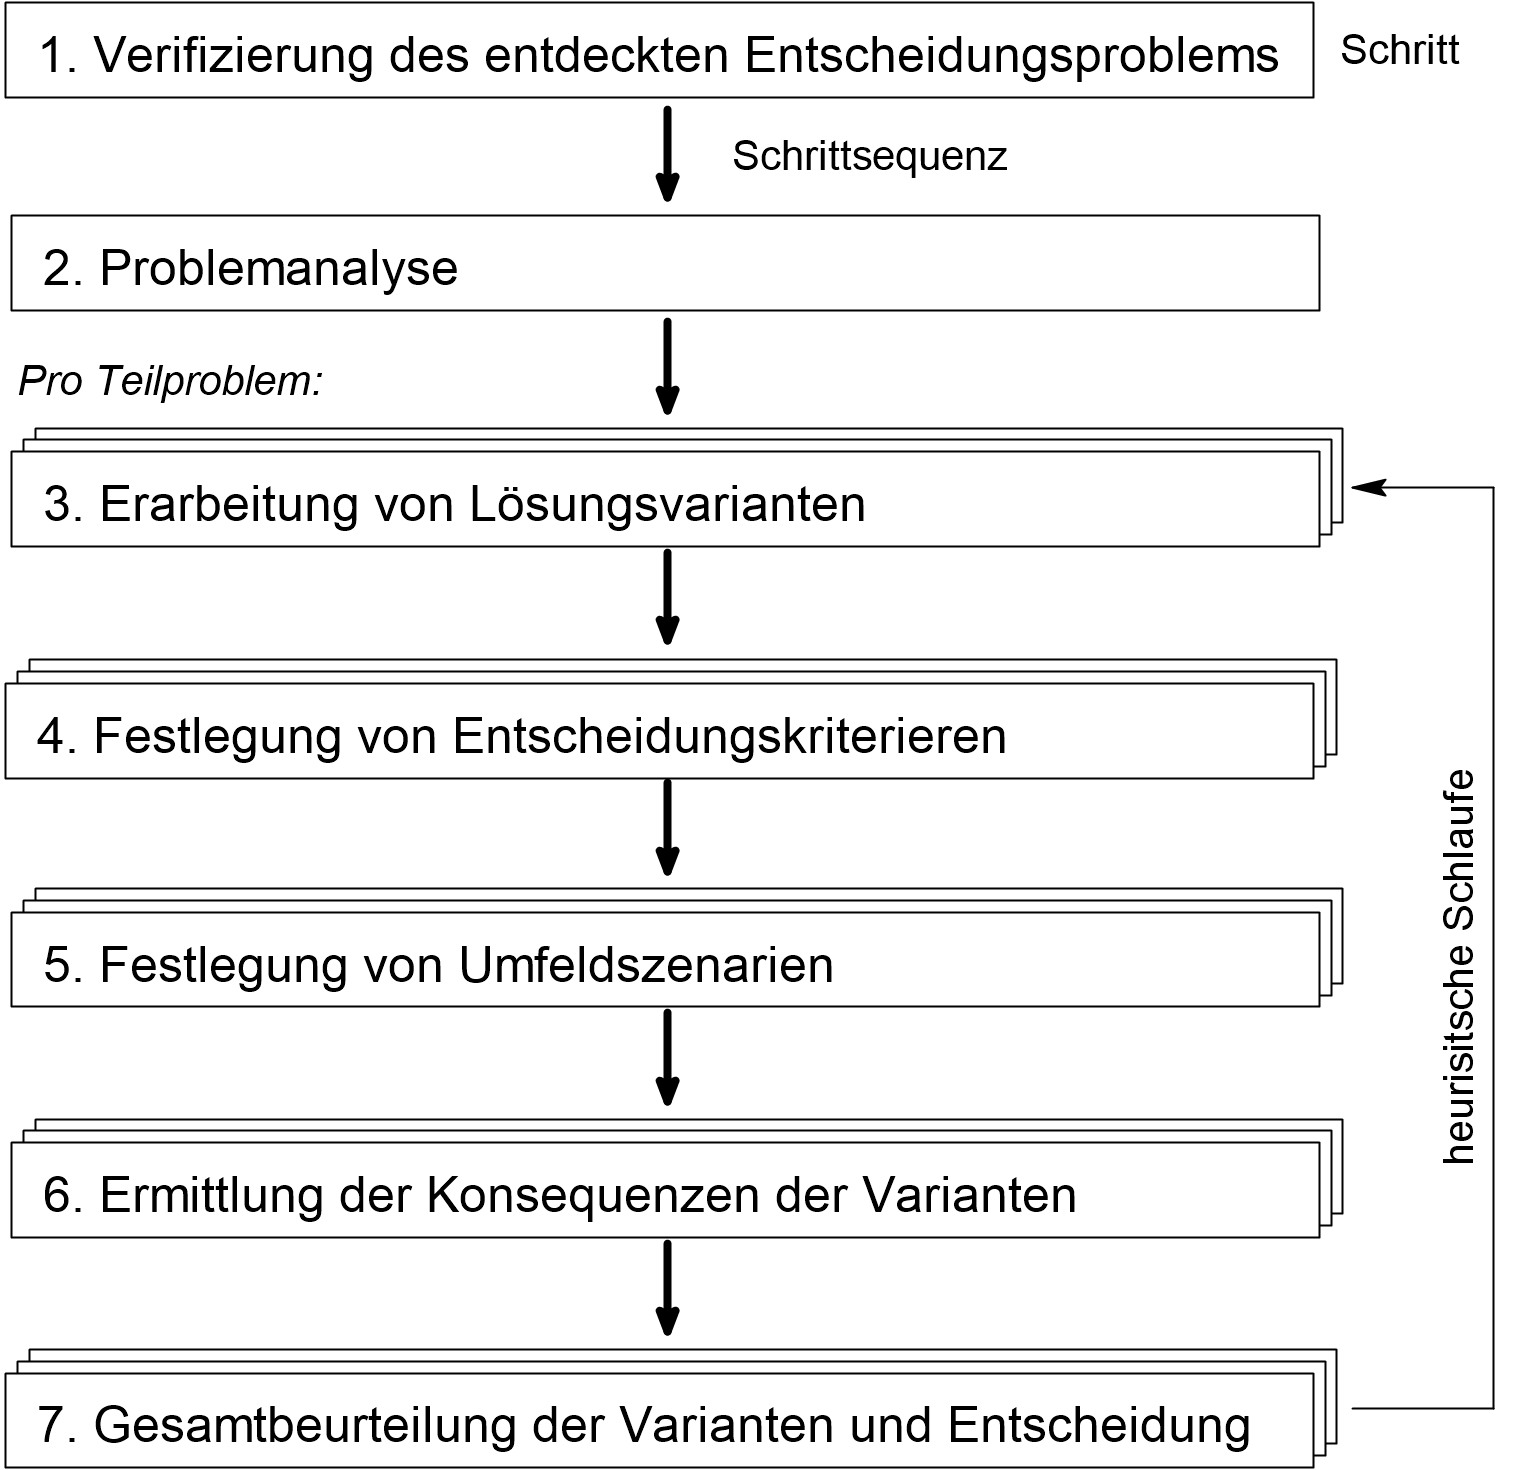
\includegraphics[width=0.5\textwidth]{img/heuristik}
	\caption{Allgemein heuristisches Entscheidungsverfahren, erstellt nach \cite{Grunig.2013}}
	\label{fig:ahev}
\end{figure}
\FloatBarrier

Werden in der Problemanalyse mehrere Teilprobleme festgestellt sind die Schritte\,3 bis 7 für jedes Einzelproblem zu durchlaufen. Die Rückführung, die durch diese Entscheidungsprozesse entsteht wird "`heuristische Schlaufe"' genannt und ist mit dem am häufigsten auftretenden Vertreter in der Entscheidungsfindung in Abbildung \ref{fig:ahev} darstellt. Solche Rückführungen der Entscheidungsschritte können in allen Prozessschritten vorkommen und somit kann es in jeder Teilaktivität zu solch heuristischen Schlaufen kommen. So kann es passieren, dass die Entscheidungskriterien unter Schritt 4 angepasst werden müssen, während bereits in Schritt 6 die Konsequenzen der Lösungsvarianten bestimmt werden. Um das Verfahren anwenden und besser verstehen zu können, werden die einzelnen Schritte des Entscheidungsverfahrens kurzerhand näher erläutert. 
\vspace*{-2.5mm}
\paragraph{Schritt 1: Verifizierung des entdeckten Entscheidungsproblems} In diesem Schritt ist zu prüfen ob die Bearbeitung des Entscheidungsproblems lohnenswert ist und in wie fern sich Soll- und Ist-Zustand voneinander abweichen und auf verlässliche Informationen zurückführen lassen. Lässt sich die Bearbeitung des Problems als lohnenswert und die Beschreibung des Soll- und des Ist-Zustandes auf valide Informationen zurückzuführen ist, gilt das Problem als verifiziert. Je nach Wichtigkeit und Dringlichkeit wird dann festgelegt wer und in welchem Zeitraum an dem Entscheidungsproblem gearbeitet werden soll. Ist keine Aussage zur Wichtigkeit und Dringlichkeit möglich wird von beiden der Worst-Case angenommen.
\vspace*{-2.5mm}
\paragraph{Schritt 2: Problemanalyse} In diesem Schritt wird die Problemstellung abgegrenzt und strukturiert. Im Zuge dieser Analyse erfolgen dann Recherchen und Ermittlungen von relevanten Informationen, um die Problemursachen festzustellen und das Problem in mehrere Teilprobleme zu zerlegen. Danach wird festgelegt welche dieser einzelnen Probleme parallel oder nacheinander bearbeitet werden können. Diese Struktur ist maßgeblich für das Vorgehen in den folgenden Schritten.\\

Die folgenden Schritte 3 bis 7 werden mit jedem Teilproblem einzeln durchgeführt und es kann gegebenenfalls zu heuristischen Schlaufen innerhalb dieser Bearbeitungsschritte kommen. Je nach vorgegebener Struktur unter Schritt 2 kann die Bearbeitung dieser Teilprobleme unterschiedlich angegangen werden.
\vspace*{-2.5mm}
\paragraph{Schritt 3: Erarbeitung von Lösungsvarianten} In diesem Schritt des Entscheidungsverfahrens werden mindestens zwei oder mehr Lösungsvarianten für das Teilproblem erarbeitet. Um den weiteren Bewertungsprozess des Entscheidungsverfahrens rechtfertigen zu können, ist bei der Erarbeitung der Varianten zu beachten, dass sich diese in wesentlichen Merkmalen und nicht nur in Details unterscheiden. 
\vspace*{-2.5mm}
\paragraph{Schritt 4: Festlegung von Entscheidungskriterien} Sind die Lösungsvarianten bestimmt, gilt es sich als nächstes die Entscheidungskriterien festzulegen anhand derer die Varianten evaluiert werden sollen. Die Beschreibung dieser Kriterien besticht dabei durch konkret definierte Maßstäbe anhand derer eine Einschätzung erfolgen kann.
\vspace*{-2.5mm}
\paragraph{Schritt 5: Festlegung von Umfeldszenarien} Dieser optionale Schritt des Entscheidungsprozesses fordert den Aktor der Entscheidung dazu auf, falls nötig, verschiedene Szenarien des Umfeldes zu beschreiben und Eintrittswahrscheinlichkeiten dafür zu definieren. In der Risiko- und Gefahrenanalysen nach dem HAZOP-Verfahren findet eine solche Beurteilung des Umfeldes beispielsweise statt. \todo{Münch nachfragen ob diese Riskotabelle nur für HAZOP galt}
\vspace*{-2.5mm}
\paragraph{Schritt 6: Ermittlung der Konsequenzen der Varianten:} Die zuvor überlegten Entscheidungskriterien und die optionalen Umweltszenarios werden mit den erarbeiteten Lösungsvorschlägen in einer Entscheidungsmatrix zusammengefasst und die sich daraus ergebenen Konsequenzwerte eingetragen. Die Konsequenzwerte werden hierbei durch eingehende Recherchen und dem Wissen und der Erfahrung des Aktors bestimmt und können daher auch einer gewissen Subjektivität unterliegen.
\vspace*{-2.5mm}
\paragraph{Schritt 7: Gesamtbeurteilung der Varianten und Entscheidung} Im letzten Schritt werden die einzelnen Lösungsvarianten in ihrer Gesamtheit beurteilt. Dafür werden irrelevante Varianten eliminiert und danach bestimmt ob für die Wahl der Lösungsvariante ein analytisches oder summarisches Vorgehen bevorzugt wird. Dies entscheidet sich dadurch ob lediglich ein (Einwertigkeit) oder mehrere voneinander unabhängige Entscheidungskriterien (Mehrwertigkeit) die Alternativen unterscheiden und ob es unkontrollierbare Situationen gibt, die für die Variantenwahl entscheidend sind. Im Normalfall kann bei komplexen Problem davon ausgegangen werden, dass diese mehrwertig sind und/oder eine gewisse Unsicherheit oder Ungewissheit der Situation in sich tragen. Laut \cite{Grunig.2013} wird daher ein analytisches Vorgehen bevorzugt bei der Hilfswerte gebildet und verrechnet werden können. Alternativ dazu können sich bei einwertigen und/oder sicheren Entscheidungen auch summarisches Vorgehen eignen, da diese durch Abwägung der Vor- und Nachteile der Varianten weniger komplex und besser interpretierbar sind. 
In der Literatur sind für die jeweiligen Vorgehensweisen verschiedene Methoden, sogenannte Entscheidungsmaximen beschrieben, welche die Überwindung von Mehrwertig, Unsicherheit oder Ungewissheit möglich machen. Eine Möglichkeit der Überwindung der Mehrwertigkeit und der Unsicherheit ist zum Beispiel die auf \textsc{Bernoulli} zurückgehende Maxime des Nutzenerwartungswertes.\linebreak
Ist die Bestimmung der Varianten für die einzelnen Teilprobleme nach analytischen oder summarischen Vorgehen erfolgt, können infolgedessen die vorgeschlagenen Varianten der Teilprobleme mit einander abgestimmt werden. Bildet sich dabei keine heuristische Schleife fällt die Entscheidung über die zu realisierende Variante.

\subsubsection{Nutzenwertmaxime}
Für das analytische Vorgehen bei der Gesamtbeurteilung der Varianten kann die Nutzenwertmaxime zur Überwindung von Mehrwertigkeit genutzt werden. Sie unterscheidet sich von der Maxime des Nutzenerwartungswertes nach \textsc{Bernoulli} durch die fehlende Einbeziehung des Erwartungswertes und überwindet somit auch keine Unsicherheiten. Das muss jedoch bei sicheren Situationen der Entscheidung keinen Nachteil mit sich bringen. Die Entscheidung einer Variante mittels Nutzenwertmaxime umfasst vier Teilaufgaben: 
\vspace*{-2.5mm}
\paragraph{Schritt 1: Umrechnung nicht-numerischer Konsequenzwerte}	\, \\
Nicht-numerische Konsequnzwerte sind anhand einer definierten Skala in Zahlenwerte umzurechnen.
\vspace*{-2.5mm}
\paragraph{Schritt 2: Umrechnung der Konsequenzwerte in Nutzenwerte} \, \\ 
Für jedes Entscheidungskriterium hat die Summe an Nutzwerten der Variante "`1"' zu betragen. Die Nutzwerte der Varianten sind dabei so zu bestimmen, dass die Nutzenwerte zwischen $0$ und 1 liegen und das die günstigste Konsequenz den höchsten Nutzenwert besitzt.
\vspace*{-2.5mm}
\paragraph{Schritt 3: Gewichtung der Entscheidungskriterien} \, \\
Die Summe der Gewichtungen der Entscheidungskriterien sollte auch an dieser Stelle wieder 1 betragen, um eine Vergleichbarkeit zu gewährleisten. Die rein subjektiven Gewichte sollten hierbei die relative Bedeutung für die Zielerreichung widerspiegeln.
\vspace*{-7.5mm}
\paragraph{Schritt 4: Bestimmung der Gesamtkonsequenzen} \, \\
Die Nutzenwerte von jedem Entscheidungskriterium werden mit ihren Gewichten multipliziert und die gewichteten Nutzenwerte pro Entscheidungskriterium addiert. Die Variante mit dem höchsten Nutzenwert entspricht dann dem Entscheidungswert.

\todo[inline]{Vielleicht noch Nutzenwerttabelle zur Veranschaulichung ergänzen ?}

\subsection{Experimentelle Untersuchungen}
Um nähere Erkenntnisse über das Verdickungsmittel TAFIGEL PUR 85 der \textsc{Münzing Chemie GmbH} zu gewinnen und eine dem Fluid gerechte Auslegung zu gewährleisten sind Untersuchungen Vorversuche unternommen worden. Hierbei ist zunächst für die strömungstechnische Auslegung die dynamische Viskosität bestimmt worden und infolgedessen untersucht worden welchen Einfluss Verdünnung und Erwärmung auf das Verdickungsmittel haben. Zudem wurden Pumpversuche mit einer Schlauchpumpe durchgeführt, um Erkenntnisse über die Pumpbarkeit zu gewinnen.

\subsubsection{Untersuchung der Temperaturabhängigkeit:} 
Durch die Verfügbarkeit eines digitalen \textsc{Brookfield DV-I Prime} Rotationsviskosimeters sind die Messungen der dynamischen Viskosität Vorort erfolgt. Um die für das Verdickermittel angegebene Viskosität von ca. \SI{35}{\pascal \second} aus dem Sicherheitsdatenblatt (vgl. \cite{MunzingChemieGmbH.2020}) zu überprüfen, wurden zunächst Untersuchungen bei \SI{20}{\celsius} nach DIN EN ISO 2555 durchgeführt. Genutzt worden sind ca. \SI{400}{\milli \liter} des Verdickungsmittels, die in ein \SI{600}{\milli \liter} Becherglas gefüllt wurden. Auf ein thermostatisches Flüssigkeitsbad ist aufgrund konstanter Raumtemperatur verzichtet worden. Gemessen wurde die Viskosität in fünf Messreihen mit einer Drehzahl von \SI{50}{\rpm} mit Spindel 7 des angegebenen Viskosimeters. Diese Spindel ist beim gegebenen Rotationsviskosimeter und \SI{50}{\rpm} für einen Viskositätsbereich von 8000 bis \SI{80000}{\milli \pascal \second} ausgelegt und wurde nach jeder Messreihe gespült und getrocknet. 
Zusätzlich ist eine Viskositätsmessung mit der gleichen Spindel, bei gleicher Drehzahl und Temperatur für ein \SI{50}{\milli \liter} Becherglas durchgeführt worden.\linebreak
Nach der Überprüfung der im Sicherheitsdatenblatt angegebenen Viskosität ist die Abhängigkeit von der Temperatur ebenfalls in Anlehnung an die DIN EN ISO 2555 untersucht worden. Auch hierbei ist, wie in der Viskositätsmessung bei \SI{20}{\celsius}, auf ein temperiertes Flüssigkeitsbad verzichtet worden und die Proben wurden stattdessen im Trockenschrank erwärmt. Nachdem die Proben aus dem Trockenschrank entnommen wurden, ist sofort die Temperatur und in direkter Folge die Viskosität gemessen worden. Möglich ist dieses Vorgehen, da sich während der Durchführung zeigte, dass in der Zeit vor und nach der Viskositätsmessung keine signifikante Temperaturänderung registriert wurde. Es sind vier Messereihen mit einem Temperaturunterschied von je ca. \SI{5}{\kelvin} durchgeführt worden.\linebreak
Neben der Viskosität wurde auch die Dichte in Abhängigkeit von der Temperatur bedacht, jedoch ist diese nicht im hauseigenen Labor der \textsc{Alberdingk Boley Leuna} bestimmt worden. Die entsprechenden Daten über den Dichteverlauf wurden beim Hersteller angefragt und sind mit einer E-Mail der Abteilung Forschung und Entwicklung beantwortet worden.

\subsubsection{Untersuchung der Verdünnungsabhängigkeit:} Da es sich beim Verdickungsmittel um ein in wässriger Lösung emulgiertes Polymer handelt wird dem Einfluss der Temperatur auch die Verdünnung bzw. die Konzentration an Aktivsubstanz betrachtet. 
Untersucht wurden hierfür die Sedimentationstabilität des Verdickungsmittels mit und ohne Verdünnung, sowie Viskositätsmessungen verschiedener Verdünnungsreihen. Letzteres wurde zum Vergleich parallel mit dem aktuell genutzten Verdickungsmittel Rheobyk-H 3300 VF der \textsc{Byk-Chemie GmbH} durchgeführt.

Geprüft wurden die dynamische Viskositäten der Verdickermittel TAFIGEL\,PUR\,85 und Rheobyk-H\,3300\,VF in Abhängigkeit von der Verdünnung erneut nach der DIN EN ISO 2555 ohne thermostatisches Flüssigkeitsbad mit einem digitalen \textsc{Brookfield DV-I Prime} Rotationsviskosimeter. Die Raumtemperatur von \SI{20}{\celsius} blieb während der Messung konstant. Die Wahl der Spindel , sowie der Drehzahl hing stark von der jeweils vorliegenden Viskositäten, dem Durchmesser des Becherglases und dem Messbereich des Viskosimeters ab. Lag eine Konfiguration des Viskosimeters außerhalb eines für die Probe nötigen Messbereiches, wurde man durch ein Blinken des Displays darauf aufmerksam gemacht. Genutzt wurden die Spindeln 4 bis 7, sowie die Drehzahlen 20, 50 und \SI{100}{\rpm} und sind für die jeweiligen Messreihen in Tabelle \ref{tab:visko_verdunnung} angegeben. Mehr zur Auswahl der Spindeln in Abhängigkeit von Drehzahl und Viskosität ist in der Tabelle \ref{tab:spindelwahl} zu finden.

% Table generated by Excel2LaTeX from sheet 'Daten'
\begin{table}[h!]
	\renewcommand*{\arraystretch}{1.2}
	\centering
	\caption{Viskositätsbereiche der verschiedenen Spindeln in Abhängigkeit von der Drehzahl, erstellt nach \cite{brookfield_31.01.2022}}
	\label{tab:spindelwahl}
	\resizebox{\textwidth}{!}{
		\begin{tabulary}{1.33\textwidth}{C|C|C|C|C|C|C|C|C}
			\hline
			\multicolumn{2}{c|}{\textbf{Spindel}}  & \textbf{1} &\textbf{2}&\textbf{3}&\textbf{4}&\textbf{5}&\textbf{6}&\textbf{7}\\
			\hline
			 \textbf{Viskosität} & \textbf{\SI{20}{\rpm}} 					&$<$500&200-2000&500-5.000&1.000-10.000&2.000-20.000&5.000-50.000&20.000-200.000\\
			 \cline{2-9}	
			 \textbf{in}& \textbf{\SI{50}{\rpm}} 							&$<$200&80-800&200-2.000&400-4.000&800-8.000&2000-20.000&8.000-80.000\\
			 \cline{2-9}	
			 \textbf{\si{\milli \pascal \second}}& \textbf{\SI{100}{\rpm}} 	&$<$100&40-400&100-1.000&200-2.000&400-4.000&1000-10.000&4.000-40.000\\
			 \hline
	\end{tabulary}
}
\end{table}%
\FloatBarrier

Für die Messreihen ist das jeweilige Verdickungsmittel zusammen mit Wasser in einem \SI{50}{\milli \liter} Becherglas vermengt worden. Aufgrund einer Knappheit an Verdickungsmittel im Labor durch das parallel getestete Sedimentationsverhalten wird bewusst ein \SI{50}{\milli \liter}-, statt einem  \SI{600}{\milli \liter}-Becherglas genutzt. Dass damit die Vergleichbarkeit mit den vorangegangenen Viskositätsmessungen vermindert wird, ist in der Diskussion der Ergebnisse unter Abschnitt \ref{sec:diskussion} berücksichtigt. Pro Verdickermittel sollten die Messungen  jeweils mit einem Massenanteil an Verdickungsmittel von \SI{100}{\percent} beginnen und in \SI{10}{\percent}-Schritten reduziert werden, sodass am Ende pro Verdickungsmittel neun Viskositätsmessungen durchgeführt wurden. Die Messung bei \SI{0}{\percent} Verdickungsmittelanteil ist nicht vollzogen worden. Auch bei diesen Viskositätsmessungen sind bei mehrfacher Anwendung die Spindeln zwischen den Messungen gespült und getrocknet worden. 

% Table generated by Excel2LaTeX from sheet 'Daten'
\begin{table}[h!]
	\renewcommand*{\arraystretch}{1.2}
	\centering
	\caption{Messparameter und Massenanteile für verdünnte Viskositätsmessungen}
	\label{tab:visko_verdunnung}
	%\resizebox{10.5cm}{!}{
		\begin{tabulary}{1.0\textwidth}{C|C|C|C|C|C|C}
			\hline
			\textbf{Nr.} & \textbf{Spindel} & $\boldsymbol{n \left[\si{\rpm}\right]}$ &\textbf{$\boldsymbol{m_\text{VD} \left[\si{\gram}\right]}$}&\textbf{$\boldsymbol{m_{\ce{H2O}} \left[\si{\gram}\right]}$}&\textbf{$\boldsymbol{m_{\text{ges}} \left[\si{\gram}\right]}$}&\textbf{$\boldsymbol{w \si{\percent}_{\text{VD}} \left[\si{\percent}\right]}$}\\
			\hline
			\multicolumn{7}{l}{TAFIGEL PUR 85}\\
			\hline
			1&4&100	&9,9&		39,6&49,5&20\\
			2&5&100	&13,3&		31,1&44,4&30\\
			3&5&100	&19,0&		28,5&47,5&40\\
			4&5&50	&24,8&		25,0&49,8&50\\
			5&5&50	&29,5&		19,9&49,4&60\\
			6&5&50	&35,7&		14,8&50,5&71\\
			7&5&20&40,0&		10,3&50,3&79\\
			8&6&20&45,0&		8,8	&53,8&84\\
			9&7&50	&50,0&		0,0&50,0 &100\\
			\hline
			\multicolumn{7}{l}{Rheobyk-H 3300 VF}\\
			\hline
			1 &5&100&5,2&47,0&52,2&10\\
			2 & 5 & 50 & 10,4&42,1&52,4&20\\
			3 &5&50&15,2&35,6&50,8&30\\
			4&5&50&22,2&32,5&54,7&41\\
			5&6&100&23,9&26,4&50,32&48\\
			6&6&50&29,0&21,5&50,5&57\\
			7&6&100&40,4&9,7&50,1&81\\
			8&6&100&49,1&0,0&49,1&100\\
			\hline			
	\end{tabulary}
%}
\end{table}%
\FloatBarrier
\tablefootnote{$n$ \dots Drehzahl, $m_{\text{VD}}$ \dots Masse an Verdickungsmittel, $m_{\ce{H2O}}$ \dots Masse an Wasser, $m_{\text{ges}}$ \dots Gesamtmasse an Lösung, $w \si{\percent}_{\text{VD}}$\dots Massenanteil Verdickungsmittel}\\

Für die Überprüfung, ob das Verdickungsmittel mit der Zeit sedimentiert, wurden \SI{150}{\milli \liter} des Verdickungsmittels TAFIGEL PUR 85 in einen offenen \SI{500}{\milli \liter} Messzylinder mit $\pm \SI{10}{\milli \liter}$ Messtoleranz gegeben. Danach ist dieser Zylinder für einen Monat unter einem Abzug stehen gelassen worden. Die Erscheinungsform des Verdickungsmittels ist zu Beginn am 08.11.2021, dazwischen am 11.11.2021 und 17.11.2021, sowie am Ende dem 08.12.2021 fotografisch dokumentiert worden.\linebreak
Darauffolgend wurde das in der Untersuchung verwendete Verdickungsmittel mit einer undefinierten Menge an Wasser verdünnt. Durch dieses Vorgehen ist der Anteil an Verdickersubstanz nun über den Feststoffanteil bestimmt und mit den noch folgenden Verdünnungs-Viskositäts-Kurven verifiziert worden. Diese Lösung wurde dann beschriftet in eine Probenflasche mit Deckel abgefüllt und über zwei Monate stehen gelassen. Hiermit soll die überprüft werden ob eine Sedimentation des Verdickungsmittel bei höherem Lösemittelanteil eintritt. Die Überprüfung der Sedimentation erfolgte lediglich optisch und wurde zu Beginn am 08.12.2021 und am Ende 08.02.2022 fotografisch dokumentiert.

\subsubsection{Pumpversuche}
Da im Laufe der Bearbeitung der Dosieraufgabe die Verarbeitbarkeit des Verdickungsmittels angezweifelt wurde und noch folgende Ausführungen die Nutzung einer Schlauchpumpe in Betracht ziehen ließen, wurden Pumpversuche mit einer \textsc{Ponndorf} Classic 25 durchgeführt. Da Hersteller solcher Pumpen für gewöhnlich die Pumpenkennlinien für Wasser angeben, konnten diese für den Polyurethanverdicker nicht genutzt werden. Stattdessen wurden die mit der Pumpe möglichen Fördermengen durch Volumen- und Zeitmessungen bei unterschiedlichen Drehzahlen gemessen und mit den angegebenen Wasserfördermengen verglichen.\linebreak
Das Setup für diese Versuchsreihen ist Abbildung \ref{fig:pumpentest} dargestellt.  Die Schlauchpumpe wurde für den Versuchsaufbau mit \SI{1}{\zoll} \textsc{Kamlock}-Anschlüssen versehen und jeweils eine ca. \SI{2}{\meter} lange Saugleitung in Form eines \SI{1}{\zoll} Schlauches mit Sauglanze, sowie eine ca. \SI{6}{\meter} langem Druckleitung ebenfalls in Form eines \SI{1}{\zoll} Schlauches angebracht. Die Sauglanze wurde für die Pumptests dann in eines der \SI{200}{\liter}-Kunststofffässer mit Verdickungsmittel gegeben und das Ende des Druckschlauches in ein leeres \SI{200}{\liter}-Kunststoff gehängt. Danach sind die Pumpversuche gestartet worden in dem am Getriebe der Pumpe die niedrigste Umdrehungsgeschwindigkeit eingestellt und der Hauptschalter der Pumpe betätigt wurde. Begannen die Rotationskörper der Pumpe sich zu drehen, konnte nun über das Getriebe die Drehzahl weiter angepasst und durch ein Sichtfenster die Anzahl der Umdrehungen der Rotationskörper innerhalb einer Minute bestimmt werden.

\begin{figure}[h!]
	\centering
	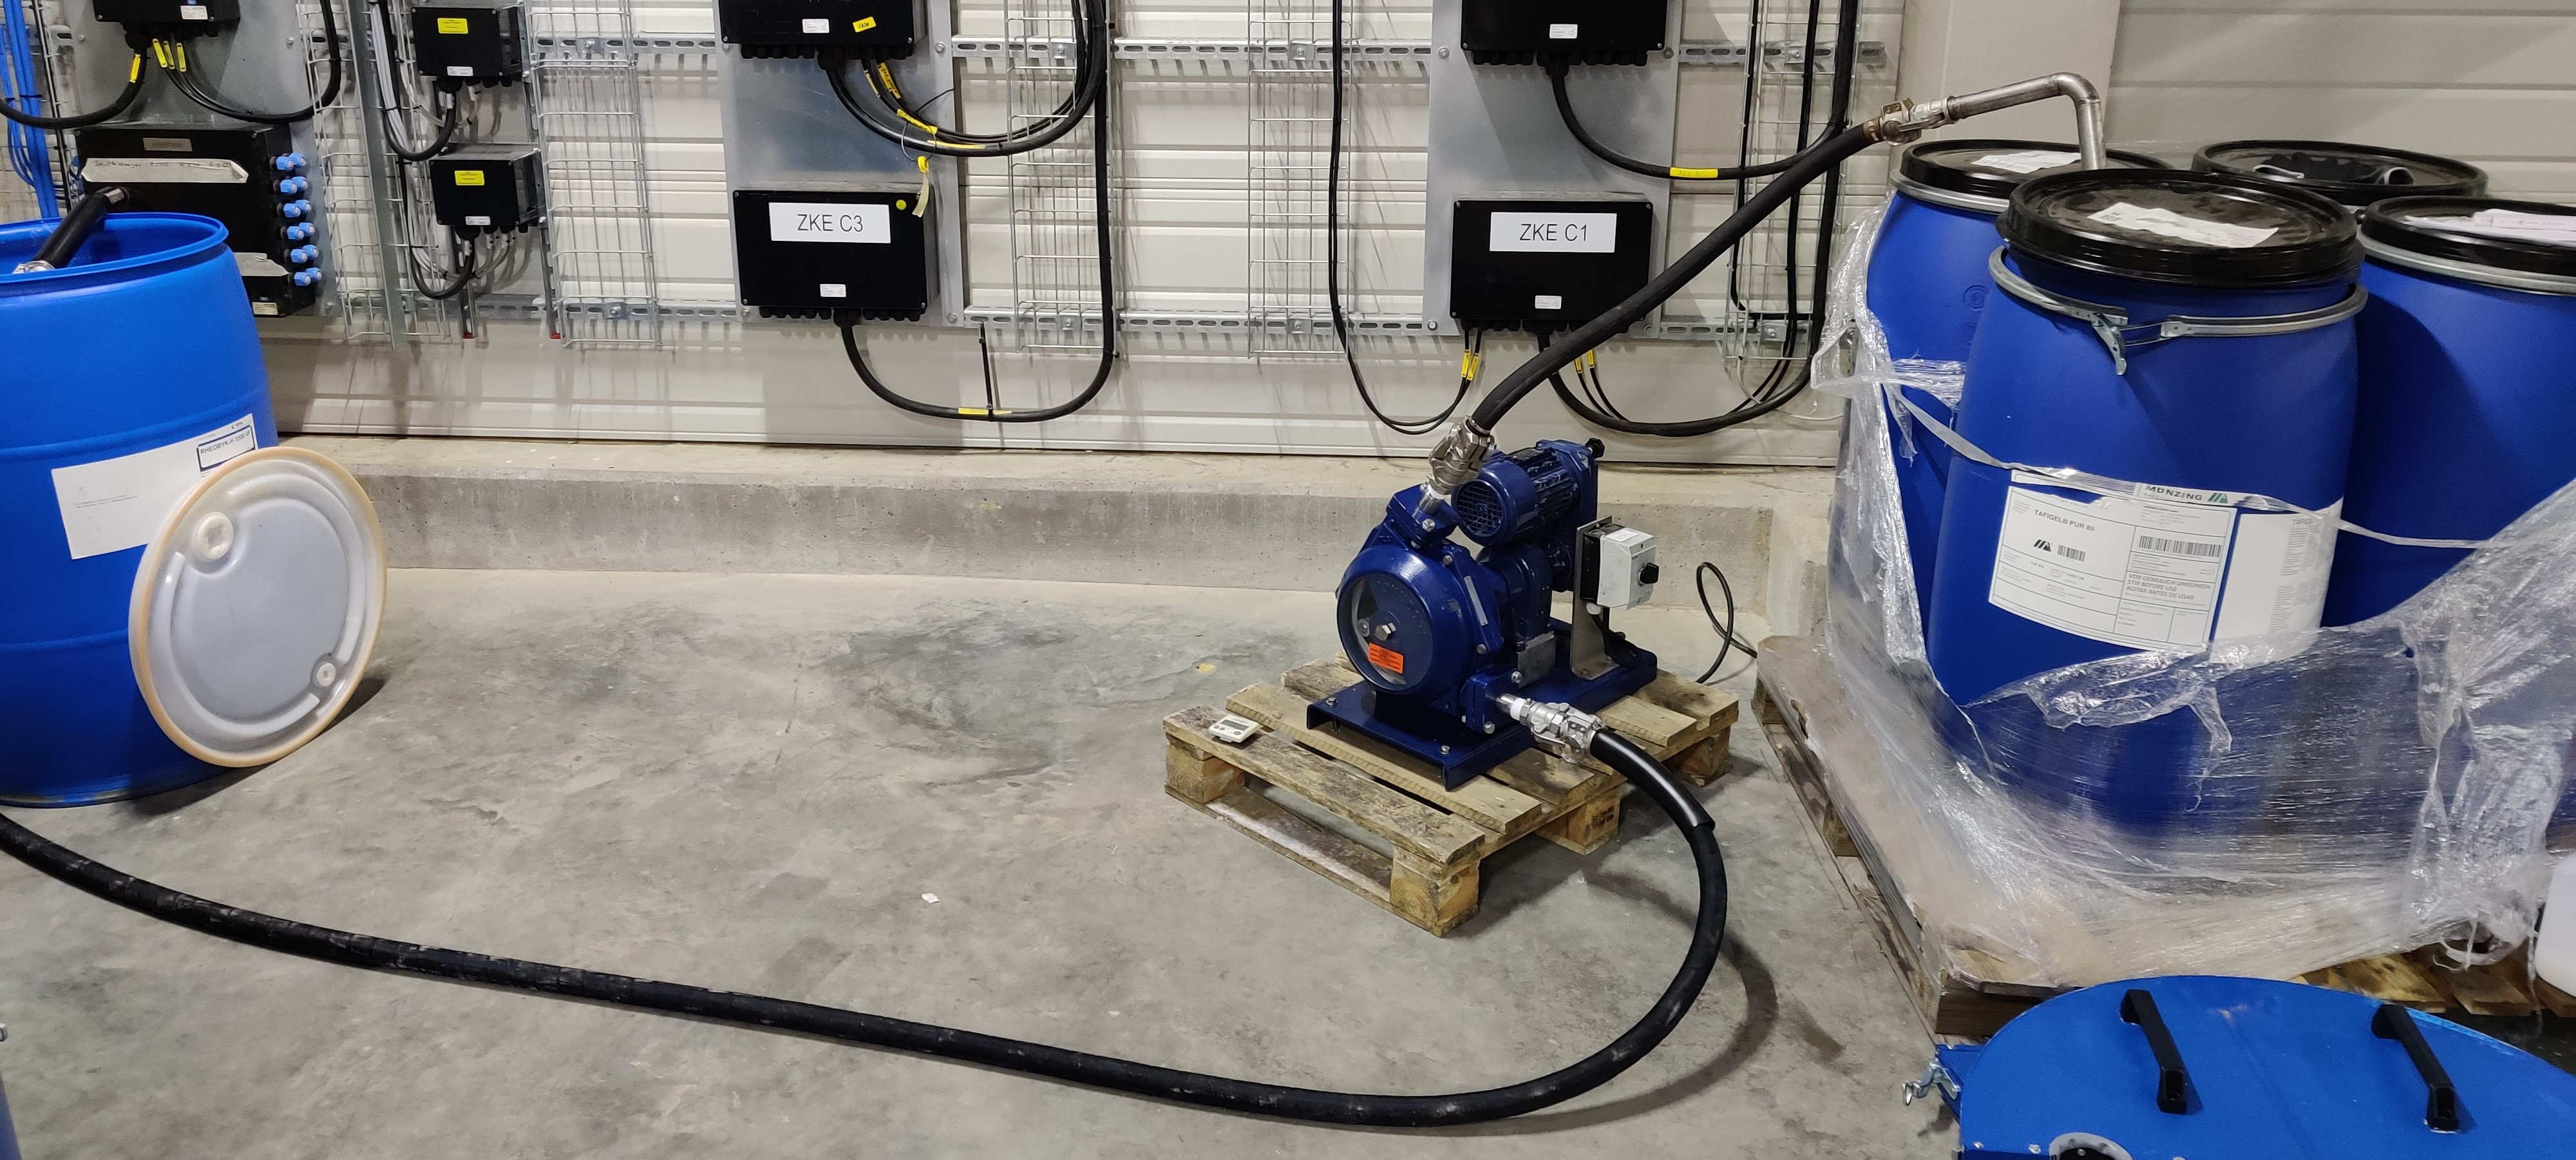
\includegraphics[width=0.75\textwidth]{img/pumpenversuch}
	\caption{Aufbau für Schlauchpumpenversuch}
	\label{fig:pumpentest}
\end{figure}
\FloatBarrier
%Ende

Sobald ein optisch konstanter Volumenstrom am Ende des Druckschlauches erkennbar war und die Drehzahl bestimmt wurde, ist die innerhalb von \SI{3}{\minute} geförderte Masse bestimmt worden. Dafür wurde das Verdickungsmittel in einer leer gewogenen \SI{1}{\liter}-Probenahmeflasche abgefüllt und danach erneut gewogen. Dieses Vorgehen ist für die Drehzahlen 33, 57, 73 und \SI{97}{\rpm} durchgeführt worden. Der Füllstand des Fasses aus dem das Verdickungsmittel gefördert wurde, sank während dieser Testreihen und wurde nicht konstant gehalten. 

\subsection{Recherchearbeit: Literaturarbeit, Fachgespräche und Angebotsanfragen}
Neben experimentelle Versuchen wurde zur Förderung des Verdickerungsmittels auch recherchiert. Zusätzlich zu den gefundenen Beiträgen von \textsc{Eberhard Schlücker} und \textsc{Gerhard Vetter} in der Literatur \cite{Vetter.2002}, wurden vor allem Gespräche mit Herstellern und Vertrieb verschiedener Pumpen- und Messtechnik, sowie dem Hersteller des Verdickungsmittels der \textsc{Münzing Chemie Gmbh} geführt. Aber auch das Studium der Datenblätter des Verdickungsmittels floß in die Recherche mit ein. \linebreak 
Eine Auswahl an angefragten Hersteller waren zum Beispiel die \textsc{AxFlow GmbH, Erich NETZSCH GmbH \& Co. Holding KG, Lutz Pumpen GmbH, Verder Deutschland GmbH \& Co. KG, FLUX-GERÄTE GMBH} für Pumpentechnik, sowie der \textsc{SCHWING Verfahrenstechnik GmbH, Endress+Hauser (Deutschland) GmbH+Co. KG, ABB Asea Brown Boveri Ltd} für Messtechnik. Die Liste an angefragten Unternehmen könnte sich an dieser Stelle auch noch weiter fortführen lassen. Grund für diese Vorgehen war die Hoffnung auf bereits vorhandene Erfahrung im Bereich der Pumpen- und Messtechnik zurück zu greifen und sich in der Umsetzung der Dosieraufgabe beraten zu lassen. Zum Teil wurden dafür auch Angebote bei den Herstellern erfragt, um auch eine preisliche Vorstellung zu bekommen. \linebreak
Beim Hersteller des Verdickermittels sind dessen Verarbeitungsmethoden zum Verdickungsmittel TAFIGEL PUR 85 erfragt und In den Datenblättern vor allem sicherheitstechnischen und physikalisch-chemische Eigenschaften herausgearbeitet worden.

\subsection{Gefährdungsbeurteilung (HAZOP-Verfahren)}
%Nur für die entschiedene Variante

\subsection{Computerunterstützes Zeichnen mit AutoCAD und QElectroTech}




